%%%%%%%%%%%%%%%%%%%%%%%%%%%%%%%%%%%%%%%%%%%%%%%%%%%%%%%%%%%%%%%%%%%%%%%%%%%%%%%%
%2345678901234567890123456789012345678901234567890123456789012345678901234567890
%        1         2         3         4         5         6         7         8

\documentclass[letterpaper, 10 pt, conference]{ieeeconf}  % Comment this line out if you need a4paper

%\documentclass[a4paper, 10pt, conference]{ieeeconf}      % Use this line for a4 paper

\IEEEoverridecommandlockouts                              % This command is only needed if 
                                                          % you want to use the \thanks command

\overrideIEEEmargins                                      % Needed to meet printer requirements.

% See the \addtolength command later in the file to balance the column lengths
% on the last page of the document

% The following packages can be found on http:\\www.ctan.org
\usepackage{cite}
\usepackage{graphicx} % for pdf, bitmapped graphics files
\usepackage{multirow}
\usepackage{csquotes}
%\usepackage{epsfig} % for postscript graphics files
%\usepackage{mathptmx} % assumes new font selection scheme installed
%\usepackage{times} % assumes new font selection scheme installed
%\usepackage{amsmath} % assumes amsmath package installed
%\usepackage{amssymb}  % assumes amsmath package installed

\title{\LARGE \bf
CoffeeBot: An Autonomous Coffee Delivery Robot
}


\author{Jason Rebello and Ian Colwell% <-this % stops a space
%\thanks{*This work was not supported by any organization}% <-this % stops a space
%\thanks{$^{1}$Albert Author is with Faculty of Electrical Engineering, Mathematics and Computer Science,
%        University of Twente, 7500 AE Enschede, The Netherlands
%        {\tt\small albert.author@papercept.net}}%
%\thanks{$^{2}$Bernard D. Researcheris with the Department of Electrical Engineering, Wright State University,
%        Dayton, OH 45435, USA
%        {\tt\small b.d.researcher@ieee.org}}%
}


\begin{document}


\maketitle
\thispagestyle{empty}
\pagestyle{empty}


%%%%%%%%%%%%%%%%%%%%%%%%%%%%%%%%%%%%%%%%%%%%%%%%%%%%%%%%%%%%%%%%%%%%%%%%%%%%%%%%
\begin{abstract}

Robotics holds tremendous potential for benefiting every domain of human life. Over the years, the focus of robotics has shifted from the design of a simple mechanism with the integration of electronics that can perform a small set of predefined tasks to complex machines capable of operating intelligently in everyday life. The process of making a robot truly autonomous requires the understanding of several key concepts. In this paper we will address the main ideas such as mapping, localization and navigation for an autonomous coffee delivery unmanned ground vehicle (UGV) in an office setting. We will present our method and compare two custom path planners (PRM and Astar) in terms of their run-time, path generated and total distance travelled to reach a desired location.

\end{abstract}

%%%%%%%%%%%%%%%%%%%%%%%%%%%%%%%%%%%%%%%%%%%%%%%%%%%%%%%%%%%%%%%%%%%%%%%%%%%%%%%%
\section{INTRODUCTION}

There is a growing need for robots to operate intelligently and adapt to their changing environment without direct human supervision. While robots can be seen operating in several situations such as exploration, search and rescue, military operations, an area where robots have truly established a foothold is in industry and hospitals.

One of the most important tasks that nurses in a hospital spend a lot of time doing is giving medications to patients. Hospitals and warehouses move an immense amount of materials through hallways, on elevators, in basements etc. This is a complex demanding internal logistics challenge that has implications of cost, quality and safety. Automating delivery of this material generates considerable savings and efficiency. It usually requires a human to make dedicated trips in order to transfer items from one place to another. This sort of thing is a waste of time for highly trained professionals, which is why a robot makes sense to have as a delivery system. 

In this paper we will present our method at developing an autonomous robot for coffee delivery to a particular room on the third floor of engineering 5. Although the project was undertaken with the task of coffee delivery the concepts employed can be used for any other autonomous delivery system as stated above. One of the significant challenges in developing an autonomous robot is its ability to effectively localize itself in a predefined map while navigating to a specific location. We will present our approach at tackling these problems and perform a comparison of our custom Probabilistic roadmap and Grid based A-star path planning techniques.

The rest of the paper is organized as follows. In section II, we present an overview of the several autonomous delivery robots in industry. Section III, describes the hardware and software used in our setup. Section IV explains the methodology used in our project which includes the navigation stack. Section V discusses results of our custom path planners and performs a comparison of the two methods. Section VI concludes our work and states methods for improvement and future work.

\begin{figure}[!ht]
	\centering
	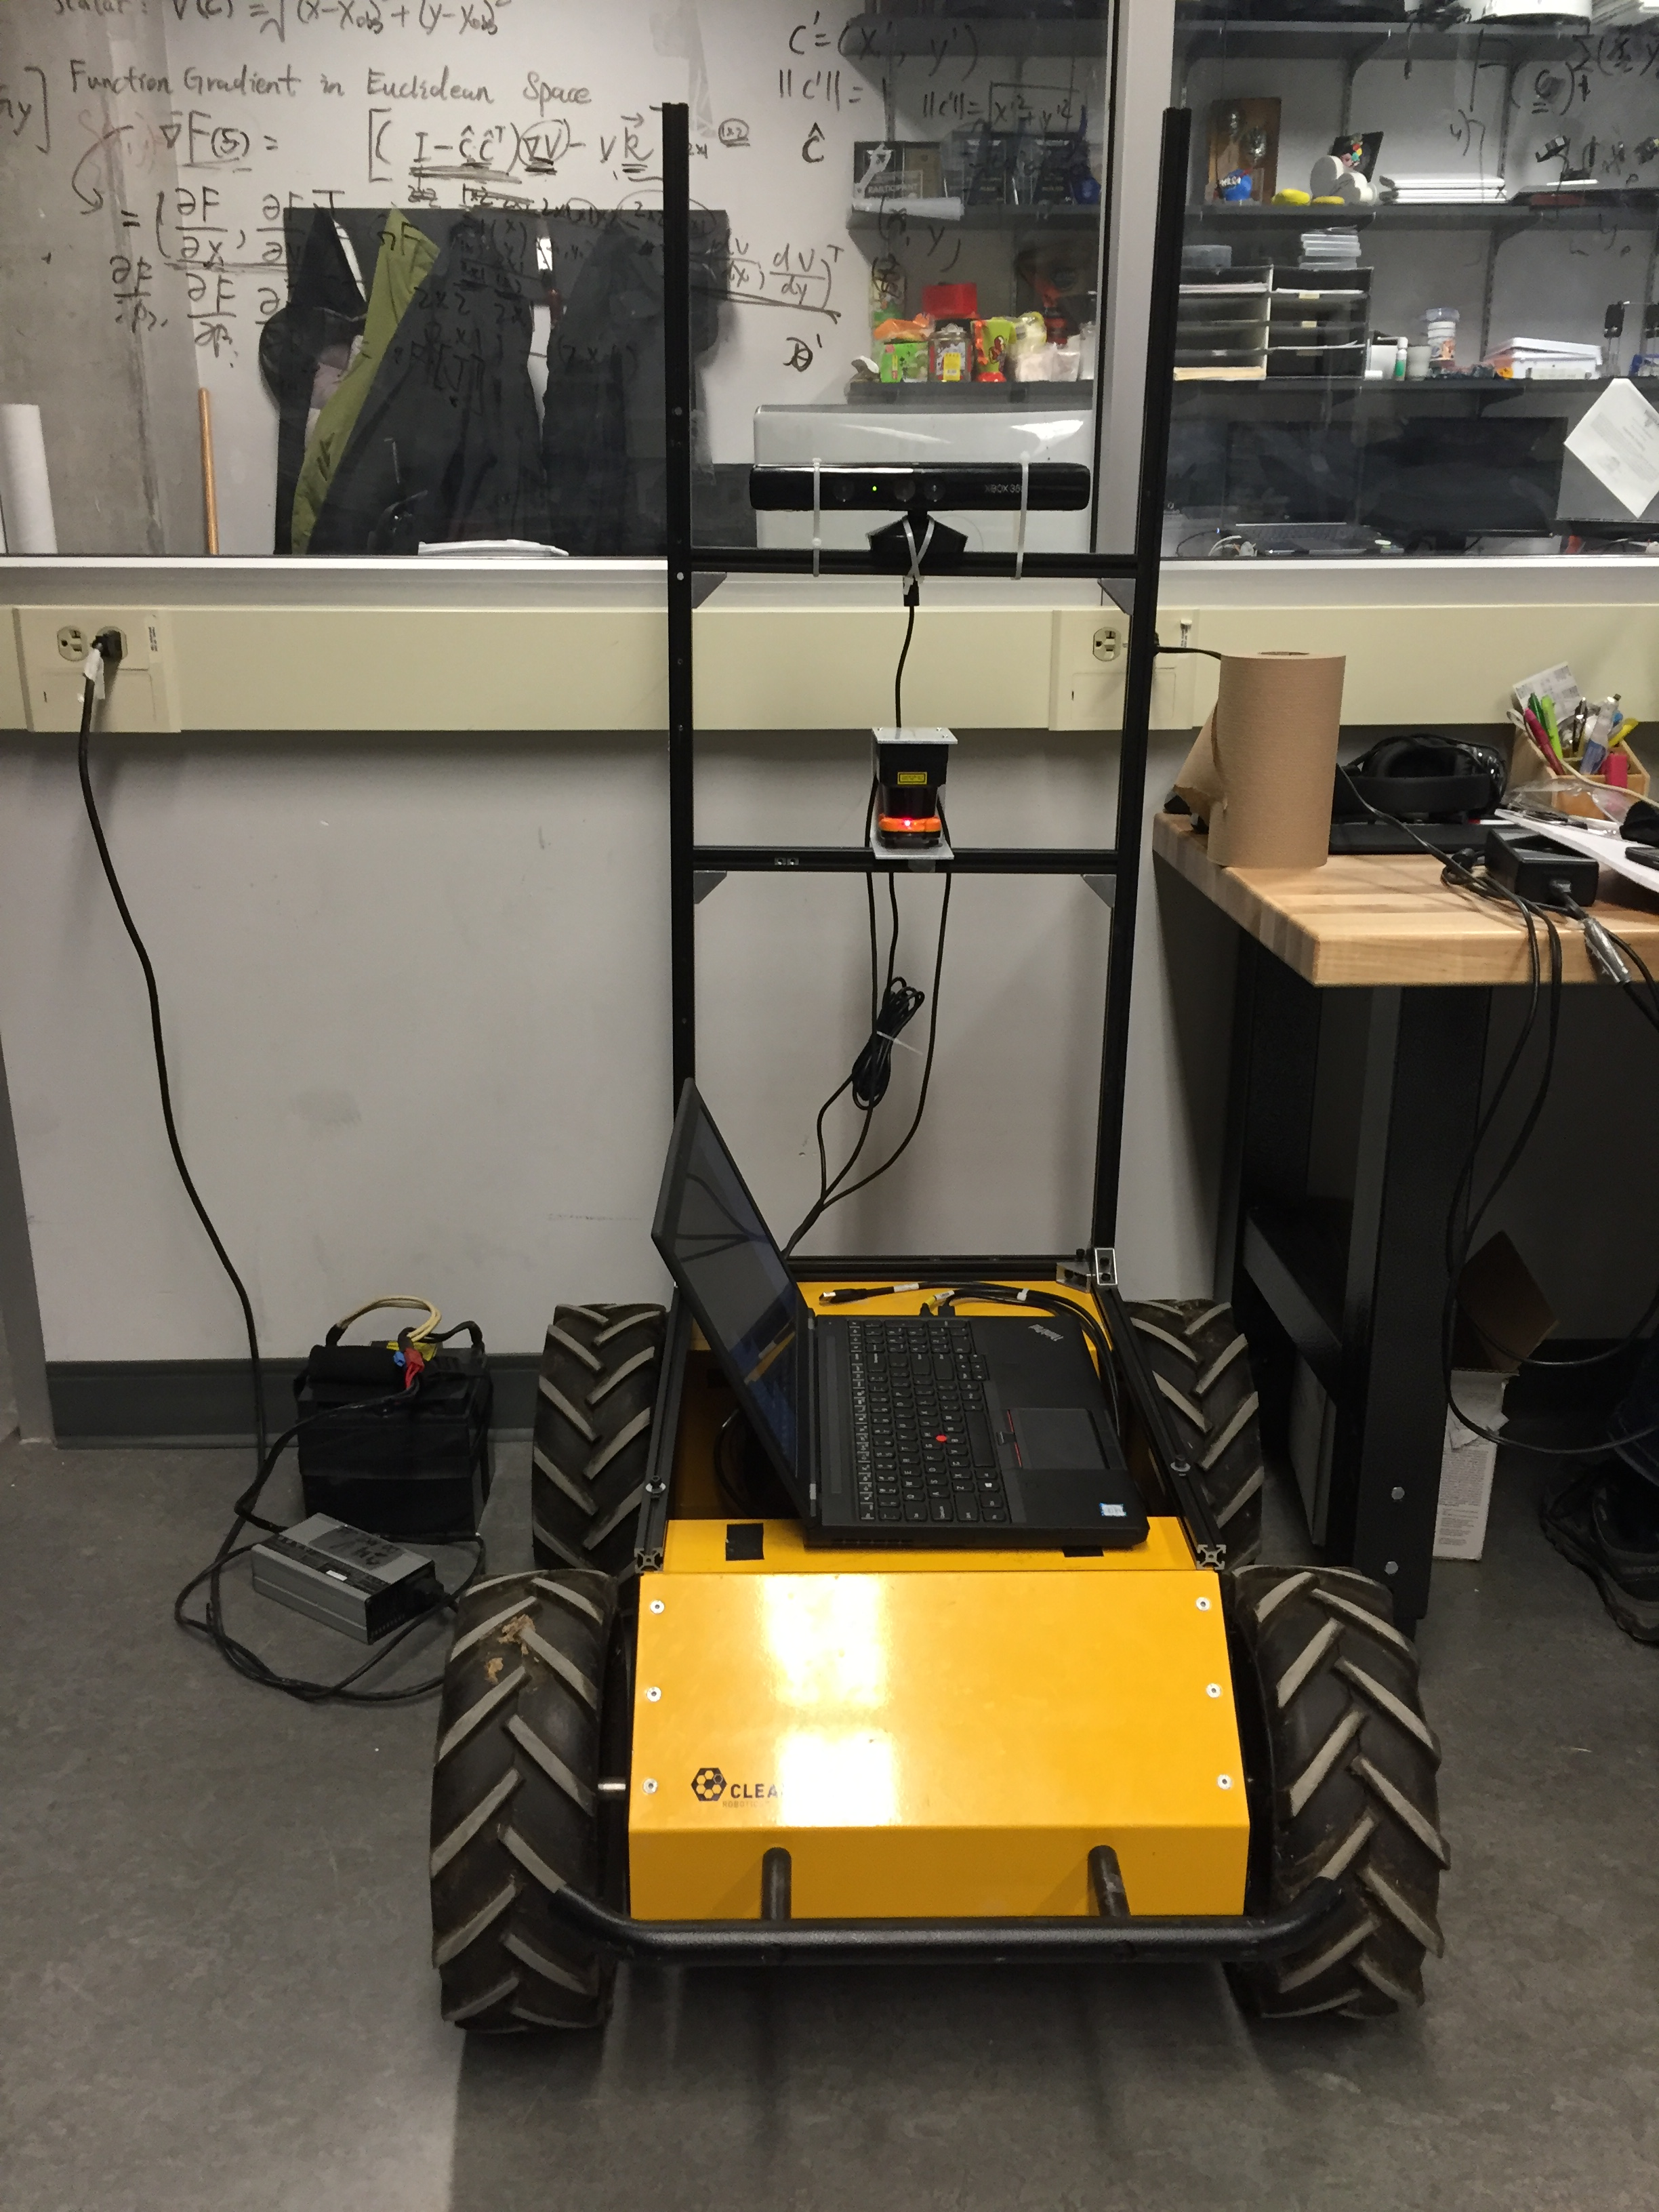
\includegraphics[width=1.0\columnwidth]{Figures/hardware_setup}
	\caption{The coffeebot.}
	\label{hardware}
\end{figure}

\section{BACKGROUND WORK}

There are a host of companies that have started developing autonomous robots for industrial tasks such as manufacturing and delivery of goods.\enquote*{Amazon} has undertaken the development of autonomous drones as part of its Prime Air delivery system. \enquote*{Google} has recently announced its desire to deliver packages from self-driving trucks. \enquote*{Clearpath Robotics} specializes in the design and manufacture of unmanned vehicle solutions for industrial and academic applications. \enquote*{Autonomous Solutions Inc} has provided unmanned vehicle hardware and software systems to clients in mining, industrial and military markets. More aligned with our project is the \enquote*{Tug} autonomous medical robot from \enquote*{Aethon} that delivers and transports medicines in an efficient and safe manner. Similarly, \enquote*{Panasonic} has been working on its \enquote*{Hospi} hospital delivery robot in order to ferry small and important objects and materials from one place to another. In most of these robots, the main sensor incorporates some sort of LiDAR (mostly 3D) that gives a fast response and at the same time provides good field of view. Due to its light weight, a camera is also frequently used as a primary tool for place recognition during localization.

\section{SYSTEM OVERVIEW}

\subsection{Hardware Used} 

The Husky unmanned ground vehicle manufactured by Clearpath Robotics was used as the mobile base. The Husky is a four wheeled skid steer system built for both outdoor and indoor use. The advantage of using this platform was its large payload capacity and power systems that can accommodate a variety of sensors. We make use of the UTM-30LX laser scanner by Hokuyo to perform scan registration for mapping and localization. Some of the main advantages of using this sensor is its high accuracy and angular resolution. The sensor returns a list of range measurements in the form of a 2D point cloud. The Microsoft Xbox Kinect sensor contains a color VGA video camera which is used to take RGB images and an infrared depth sensor that returns a 3D point cloud to form a complete RGB-D image. A Lenovo Thinkpad P50 laptop was used as the main host system for the coffeebot while a wireless Logitech handheld controller was used for test driving the robot. The complete hardware setup is shown in Figure \ref{hardware}. 
	
	\begin{figure}[!ht]
		\centering
		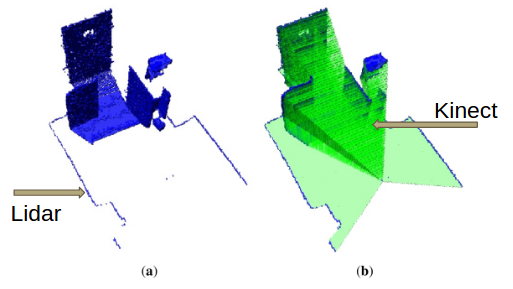
\includegraphics[width=1.0\columnwidth]{Figures/lidarKinect}
		\caption{(a) and (b) show data received from the sensors }
		\label{hardware}
	\end{figure}

\subsection{Software Used}

ROS (Robot Operating System) provided a convenient framework to build the coffeebot system using both existing open source ROS packages and the newly created coffeebot package. The important ROS packages used with the coffeebot are briefly mentioned below. An overview of the system architecture is then discussed.

\subsubsection{RTAB-Map}

This package was used as our main tool for map generation and localization in the environment. RTAB-Map stands for "Real-Time Appearance-Based Mapping" and is a RGB-D Graph-Based SLAM approach based on an incremental appearance-based loop closure detector~\cite{rtabmap2014}. The loop closure detector uses a bag-of-words approach to determinate how likely a new image comes from a previous location or a new location. When a loop closure hypothesis is accepted, a new constraint is added to the map's graph, then a graph optimizer minimizes the errors in the map. A memory management approach is used to limit the number of locations used for loop closure detection and graph optimization, so that real-time constraints on large-scale environments can be met. This package was used to generate a 3D point cloud of the environment and a 2D occupancy grid map for navigation.

\subsubsection{ROS Navigation Stack}

The ROS navigation stack is a set of ROS packages designed for moving a robot autonomously through the environment. The stack primarily consists of cost map generation for obstacle avoidance and path planning/execution for moving the robot. The ?move\_base? ROS node was used to tie all the navigation stack functions together and issue commands to drive the robot. 

\subsubsection{Coffeebot}

A new ROS package was created for the coffeebot project which consisted of three main parts. The first part is composed of launch files that were used for running the simulations and other packages needed for mapping, localization and planning. Second, a ROS service was created to issue navigation goals based on room number requests. Third, a global path planner was written as a plugin to the navigation stack. Each part will be covered in more detail in the corresponding section of this report. 

\subsubsection{RViz}

RViz was used as a visualization tool for data passed through various ROS topics. RViz has gained popularity due to its easy to configure capabilities. Custom configurations were created specifically for the coffeebot in order to make debugging quicker and easier. 

Figure \ref{software_architecture} is a simplified architecture describing the system while in navigation mode. Figure \ref{transform_tree} shows the relevant transforms of the system. As can be seen from the figure, the RTAB-Map node receives input from the laser scanner, kinect, and the odometry measurements from the Husky. RTAB-Map uses this data to estimate a position of the coffeebot relative to the predefined map. Once the first successful feature match (loop closure) is detected, RTAB-Map publishes the occupancy grid and localizes the robot within the map.  The navigation stack then transforms this occupancy grid into a static global cost map. The navigation stack also creates a local costmap that is updated four times a second using data from the Kinect and laser scanner. Using both laser scanner and kinect data allows the robot to avoid obstacles that do not appear in the plane of the laser scanner. 

A global path is generated using a global path planner and only takes into account the global cost map. Once the global path is generated through the global costmap, a local planner generates trajectories through the local costmap that track the global path. If the local planner encounters an obstacle that was not present in the global cost map, a new plan is generated. Finally, the local trajectories are then sent directly to the ?move\_base? node to be executed by the husky. 

	\begin{figure}[!ht]
		\centering
		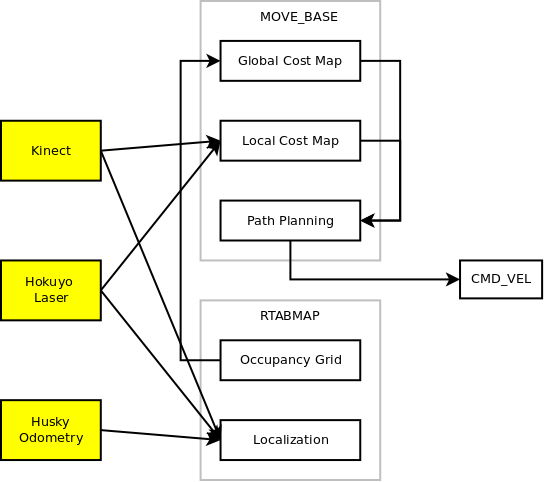
\includegraphics[width=1.0\columnwidth]{Figures/ROS_node_diagram}
		\caption{The simplified software architecture of the coffeebot.}
		\label{software_architecture}
	\end{figure}
	
	\begin{figure}[!ht]
		\centering
		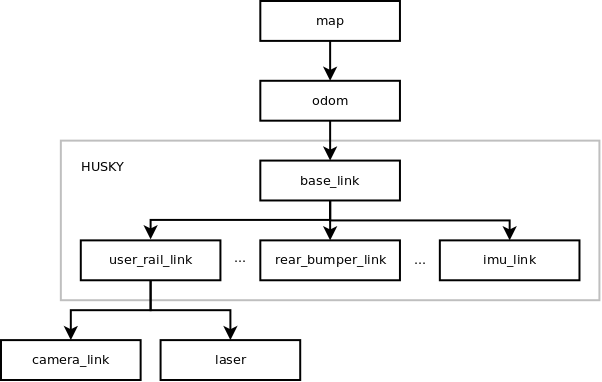
\includegraphics[width=1.0\columnwidth]{Figures/ROS_TF_diagram}
		\caption{The transforms of the coffeebot.}
		\label{transform_tree}
	\end{figure}

\section{Methodology}

\subsection{Mapping}

Autonomous robots operating in real life settings must be able to navigate in large, unstructured, dynamic and unknown spaces. To do so they must build a map of their operating environment. A map of the 3rd floor of Engineering 5 was built with the help of RTAB-Map as described in Section 3 while utilizing g2o and vertigo. The ?generalized graph optimization? (g2o) framework is an open-source C++ framework for optimizing graph-based nonlinear error functions. Vertigo is a C++ extension that enables g2o to solve pose graph SLAM problems in 2D and 3D despite a large number of false positive loop closure constraints. RTAB-Map mainly relies on the detection of ORB (Oriented FAST and Robust BRIEF) features in order extract visual words from the scene. Since the robot is constrained to operate in a single plane, the transformation can be refined with 2D iterative-closest-point (ICP) optimization using laser scans. With the help of ICP an occupancy grid map is generated. This grid map will then be used to generate the static global cost map during path planning. However, as the response from the laser scanner becomes unreliable due to poor reflection from glass surfaces, a static map using the floor plan of the building was published. This static map will be used to generate the global cost map as shown in the results section.


\subsection{Localization}

Once a map of the environment is completed, it is essential to be able to localize the robot within the existing map each time the robot is restarted. Without reliable localization, the previously generated map is useless for navigation purposes. Fortunately, RTAB-Map includes a localization mode that works very similar to the mapping mode. In localization mode, feature matches are detected (Figure \ref{localization}) between the saved image library and the input from the RGB-D camera (kinect). If sufficient matches are found then an estimate is made on the position of the robot within the map. This is very similar to the loop closure detection performed in mapping mode, except that no new constraints are added to the graph. Once the first successful feature match (loop closure) is detected, the original map reference frame is established with regard to the current odometry frame which leads to localization of the robot. see Figure \ref{transforms}

	\begin{figure}[!ht]
		\centering
		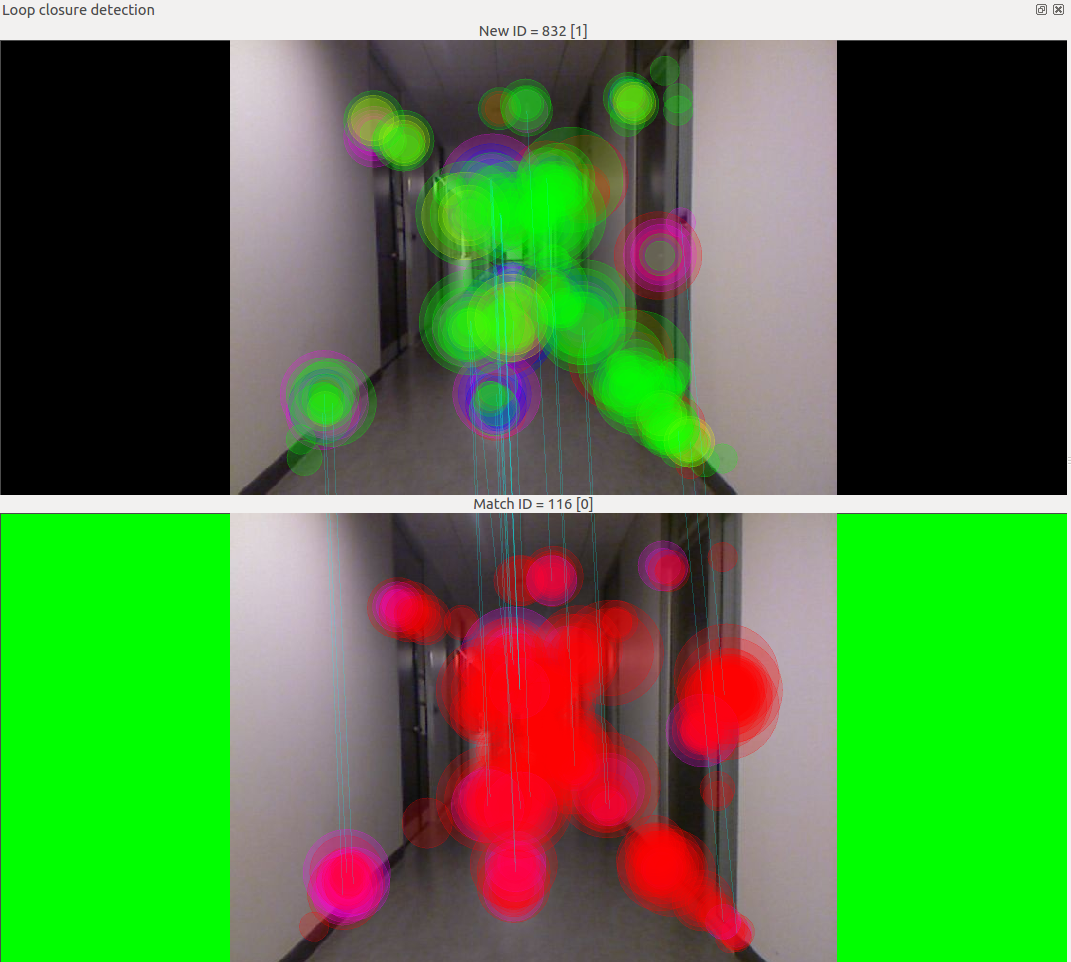
\includegraphics[width=1.0\columnwidth]{Figures/loop_closure}
		\caption{A successful feature based loop closure.}
		\label{localization}
	\end{figure}

	\begin{figure}[!ht]
		\centering
		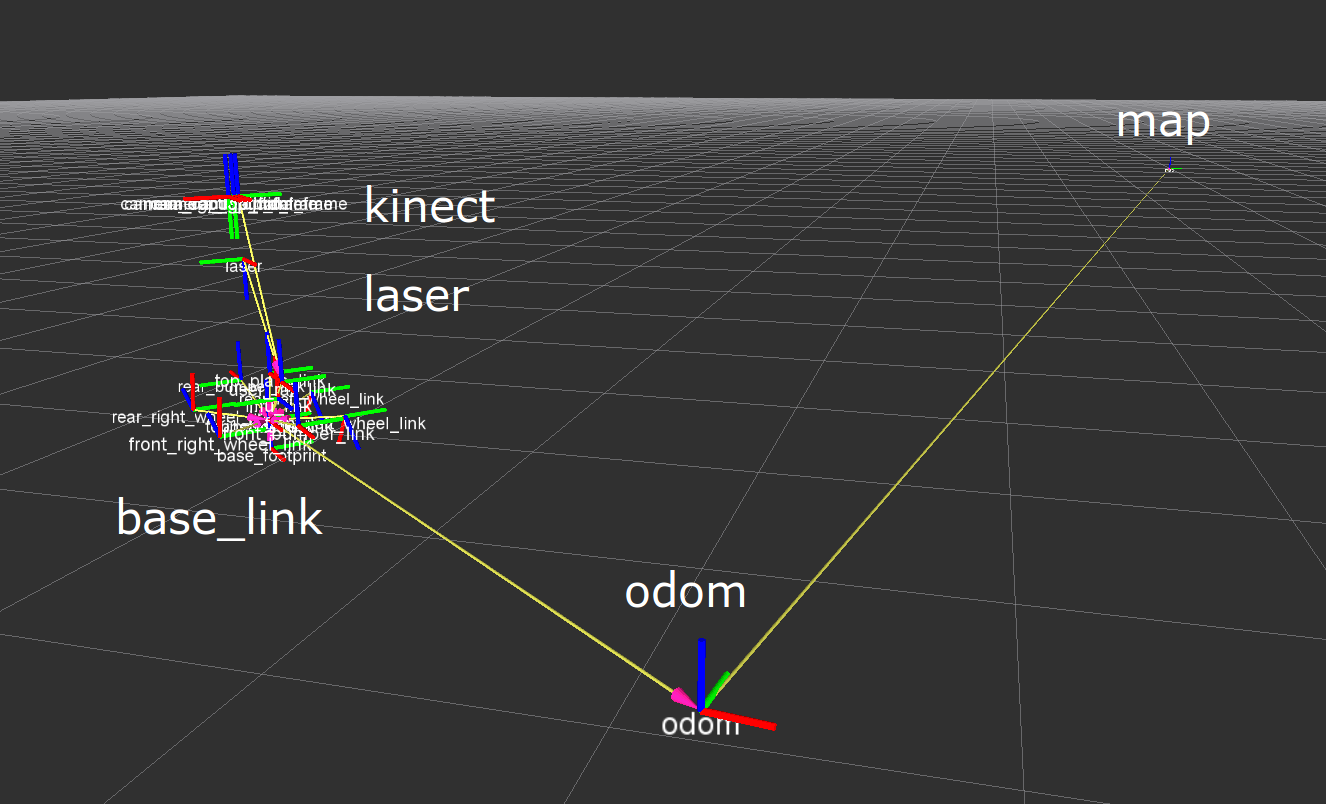
\includegraphics[width=1.0\columnwidth]{Figures/Transforms}
		\caption{The Coffeebot transforms with respect to odom and map.}
		\label{transforms}
	\end{figure}

\subsection{Planning/Navigation}

The navigation stack was used for path planning and navigation of the Coffeebot. The stack mainly consists of both a local and global costmap and a local and global path planner. The global costmap is generated from the predefined occupancy grid and the local costmap is generated live based on sensor data. A small ROS service was also created that issues goal locations based on room number requests. The service simply runs in a terminal and only takes one request at a time. As part of the navigation to various rooms, two global path planning algorithms were developed and compared. Both planners were created as global planner plugins to the ROS navigation stack for easy integration with ROS.

\subsubsection{Costmaps}

The local costmap is limited in size and is centered around the robot. This ensures dynamic objects seen in the past are not saved when returning to the area the object was first detected. Both local and global costmaps are generated using a decaying cost inflation technique. This technique assigns the highest cost to detected objects then assigns gradually lower costs out to the specified inflation radius where a cost of zero is assigned which represents free space. The 2D planar size of the robot is called the 'footprint' and is considered when building the costmaps. The dimensions used for the husky is 1 meter long and 0.65 meters wide. In Figure \ref{global_costmap} below, yellow represents an occupied cell in the occupancy grid, Aqua represents a location where the robot is definitely in collision (based on the robot footprint), Red represents a location where the robot may be in collision depending on the orientation of the robot, and Blue represents a buffer zone to keep the robot away from obstacles.

	\begin{figure}[!ht]
		\centering
		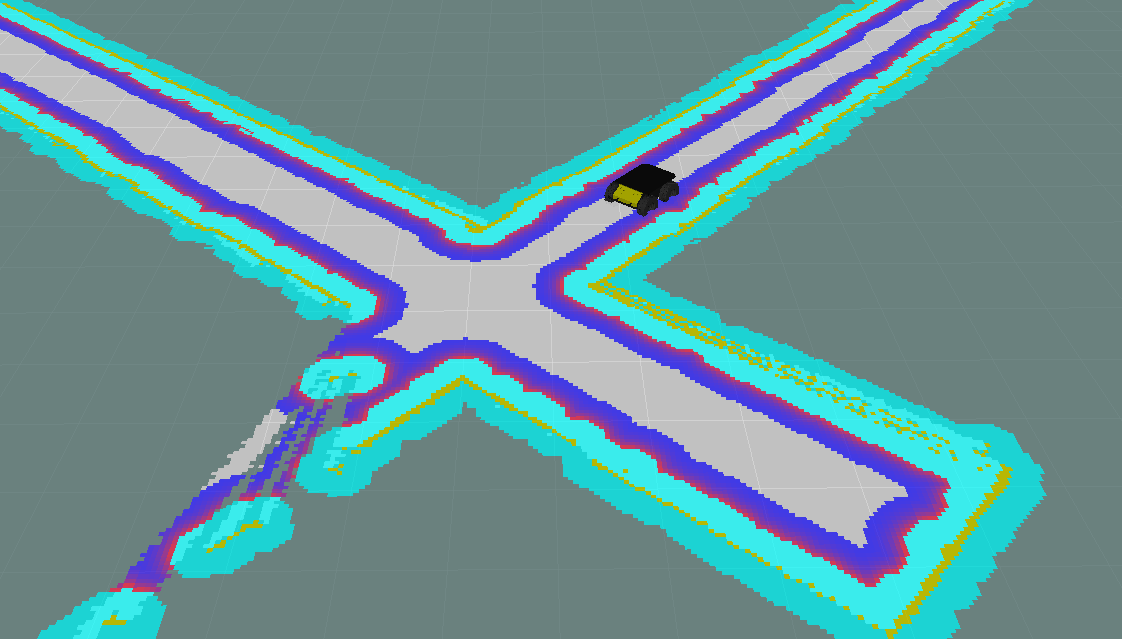
\includegraphics[width=1.0\columnwidth]{Figures/global_costmap}
		\caption{The global costmap with costs shown in colour.}
		\label{global_costmap}
	\end{figure}

\subsection{Global PRM Planner}

A custom global planner was created to generate paths for the coffeebot. The planner utilized a global costmap provided by the navigation stack to find paths between start and goal locations while avoiding areas of cost. The Probabilistic Roadmap (PRM) technique was utilized to generate a path. Creating a Probabilistic Road Maps starts with randomly sampling either the configuration space of the robot or the physical environment of the robot. While the Husky is non-holonomic, it is able to turn on the spot. For this reason, and to avoid unnecessary over complication, it was decided to sample over the environment space instead of the configuration space. Each random sample consisted of a world coordinate on the global cost map (both an X and Y position in meters). As each sample is created, the corresponding cell of the costmap is checked for a cost. If the cost is less than the allowable cost threshold then the sample is added to a list of milestones. The start and goal locations are also added as milestones if they are located in cells below the cost threshold. The completed milestone list is then iterated over to find the 20 nearest milestones to each milestone. A line to each of the nearest milestones is traced over the costmap using the bresenham line algorithm. While the line is being traced, each costmap cell in the line is checked to determine if the cost of the cell is greater than the cost threshold. The lines between milestones that can be traced without passing over costly cells are then added as edges in the roadmap (red lines in Figure \ref{PRM_planner}). Once all the available edges are created a graph based A-Star search algorithm is employed to find the shortest path through the network. The final step of the path generation is path refinement. The path returned by A-Star is then refined by attempting to skip nodes in the graph. Starting from the goal node and working back, the same bresenham line cost checking as mentioned earlier is used to check the line, or 'shortcut', between the goal node and the third-from-last node. If this line is found to be clear of costs then the second-from-last node is dropped from the path. This process repeats until every 'shortcut' in the path results in traversing a cell of cost.
Finally, the refined path (green line in Figure \ref{PRM_planner}) is sent back to the move\_base node in the form of geometry\_msgs type ROS messages to be tracked by the local planner. For debugging purposes, the network is also published using visualization\_msgs type ROS messages for easy display in RViz. 

	\begin{figure}[!ht]
		\centering
		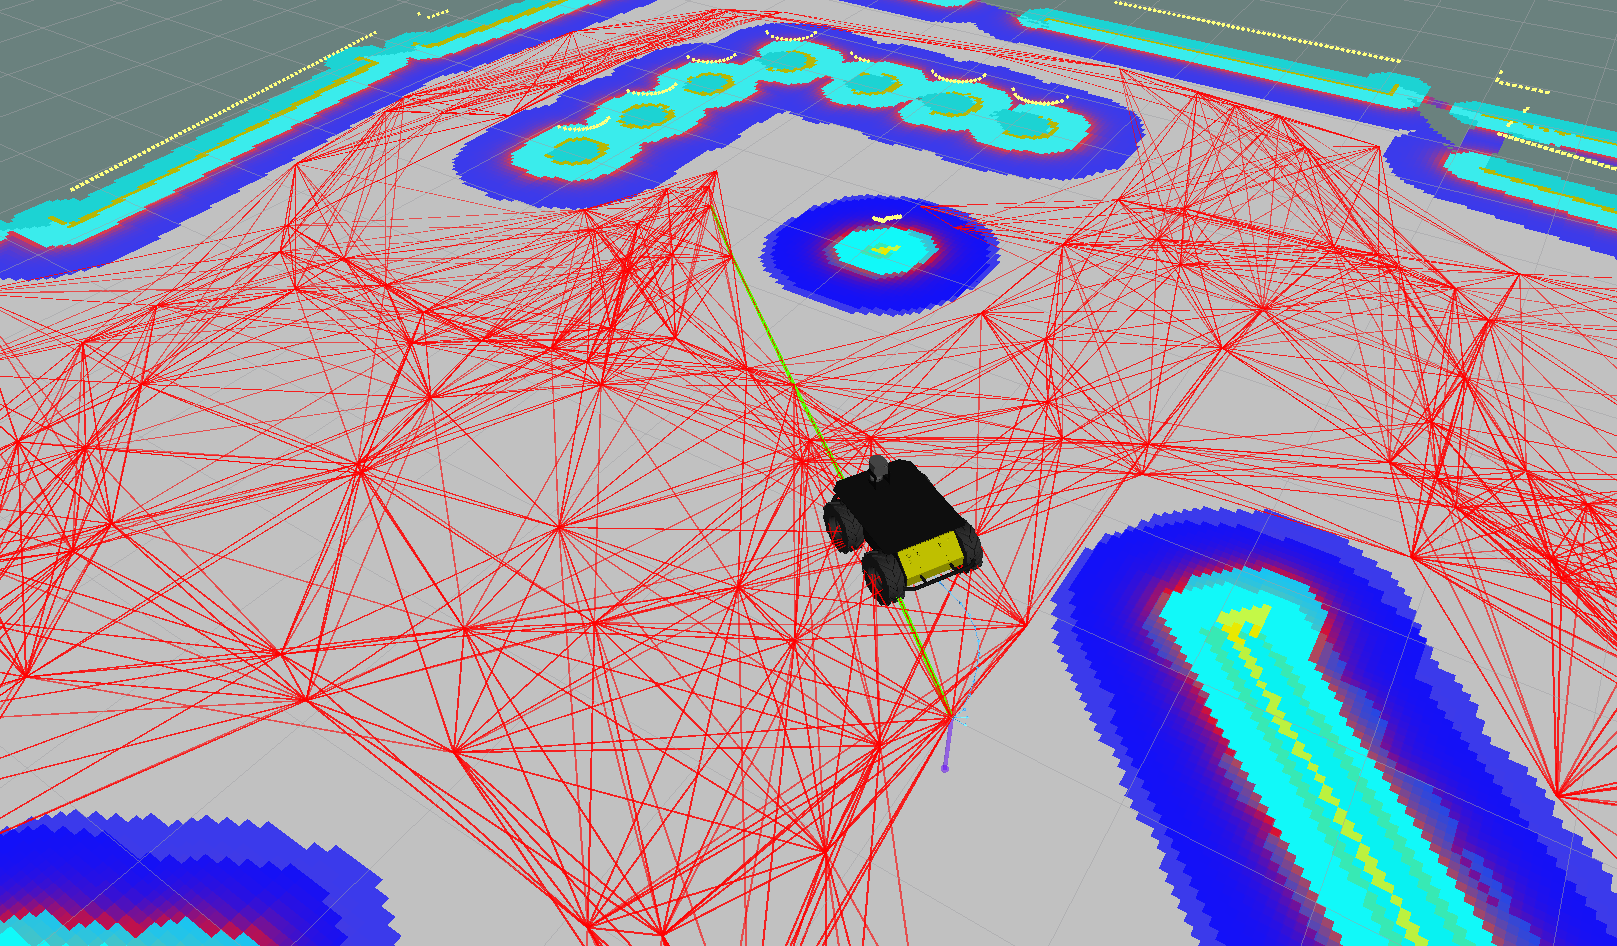
\includegraphics[width=1.0\columnwidth]{Figures/PRM_CloseUP}
		\caption{The PRM planner as seen in RViz.}
		\label{PRM_planner}
	\end{figure}

\subsection{A* Global Planner}

While the PRM method performs A* on a set of sampled points, the grid based method expands each cell from the start to the goal node based on a certain cost. The A* algorithm combines features of uniform-cost search and pure heuristic search to efficiently compute optimal solutions. A* algorithm is a best-first search algorithm in which the cost associated with a node is f(n) = g(n) + h(n), where g(n) is the cost of the path from the initial state to node n and h(n) is the heuristic estimate or the cost of the path from node n to the goal. Thus, f(n) estimates the lowest total cost of any solution path going through node n. At each point a node with lowest f value is chosen for expansion. Ties are broken randomly. The algorithm terminates when a goal is chosen for expansion. A* algorithm guides an optimal path to a goal if the heuristic function h(n) is admissible, meaning it never over-estimates the actual cost. 

\section{RESULTS}

\subsection{Mapping and Localization}

A map of the third floor of Engineering 5 was completed. This map includes a 2D occupancy grid as well as an RTAB-Map database which consists of a 3D point cloud and graph based image library. The resulting occupancy grid is shown below in Figure \ref{third_occ_grid} and a portion of the 3D point cloud is shown in Figure \ref{third_point_cloud}.

	\begin{figure}[!ht]
		\centering
		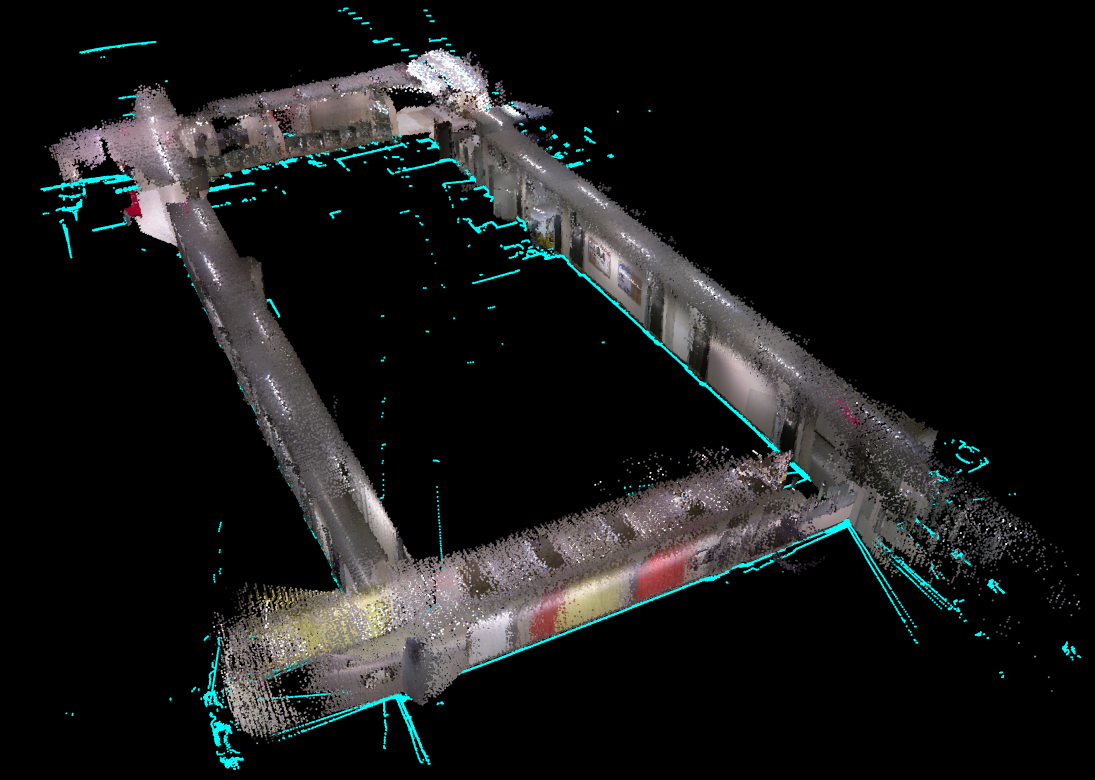
\includegraphics[width=1.0\columnwidth]{Figures/3rdfloor_point_cloud}
		\caption{The 3D point cloud map of the third floor of E5.}
		\label{third_point_cloud}
	\end{figure}
	
	\begin{figure}[!ht]
		\centering
		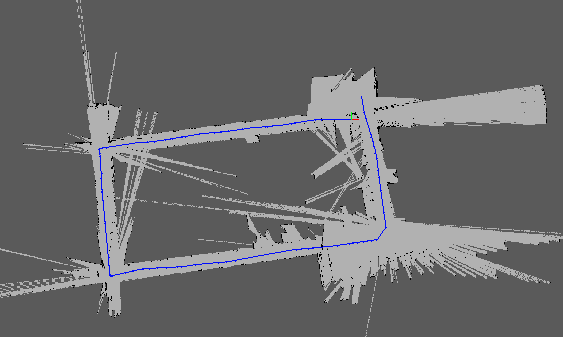
\includegraphics[width=1.0\columnwidth]{Figures/3rd_occupancy_grid}
		\caption{The occupancy grid map of the third floor of E5.}
		\label{third_occ_grid}
	\end{figure}
	
\subsection{Global Path Planning Comparison}

The two global path planners were tested and compared using the gazebo simulation environment. Two different costmaps were used in the tests. One costmap was generated from a floorplan of the third floor of Engineering 5 and another was generated from the Husky playpen demo. The resulting timing and path lengths of the two planners are compared below in Table \ref{compare_table}.  

\begin{table}[h]
\caption{The comparison results of the two global path planners tested on two different environments.}
\label{compare_table}
\begin{center}
\begin{tabular}{l|c|c|c|c|}
\cline{2-5}
                                    & \multicolumn{2}{c|}{\textbf{Time to Generate Path (ms)}} & \multicolumn{2}{c|}{\textbf{Path Length (m)}} \\ \hline
\multicolumn{1}{|l|}{\textbf{Test Costmap and Goal}} & \textbf{Grid A*}    & \textbf{PRM}    & \textbf{Grid A*}     & \textbf{PRM}     \\ \hline
\multicolumn{1}{|l|}{E5 Third Floor - 1} & 53.777 & 47.252 & 48.599 & 48.093 \\ \hline
\multicolumn{1}{|l|}{E5 Third Floor - 2} & 33.363 & 29.229 & 23.189 & 22.473 \\ \hline
\multicolumn{1}{|l|}{Husky Playpen - 1} & 90.177 & 12.885 & 13.332 & 13.778 \\ \hline
\multicolumn{1}{|l|}{Husky Playpen - 2} & 32.581 & 3.266 & 8.591 & 8.819 \\ \hline
\end{tabular}
\end{center}
\end{table}


\section{CONCLUSION}

After running several tests, we found that while RTAB-Map is a good out-of-the-box tool for mapping, it does not provide a robust solution under various lighting conditions. This can be attributed to the fact that RTAB-Map relies mainly on the kinect sensor which is known to fail in these situations. A way to tackle this issue would be to employ the use of wide field of view cameras with some form of pre-filtering process such as histogram equalization.
Although the Hokuyo laser scanner provides range measurements at a high update rate, it is limited to a 2D plane. Since obstacles below this plane fail to be detected, placement of the Hokuyo on the robot becomes critical. The use of a multibeam 3D laser scanner would help solve this problem.
RTAB-Map relies on ORB detector and descriptor for recognizing features in the environment. While it detects a number of features, applying SIFT/SURF detectors would help improve matching. It was found that odometry readings from the Husky were more reliable at high speeds and travelling in a straight line as compared to readings observed during rotation.

\section{FUTURE WORK}

In the future there will be a need for teams of small, agile autonomous robots to perform intelligence, surveillance and reconnaissance (ISR) missions. As a result, we would like to extend the ground vehicle to communicate with aerial vehicles such as quadrotors. Person following and tracking is another area of interest. In industry most robots are programmed to perform specific tasks, however, if the robot can track a \enquote*{master} it will have the ability to learn new responsibilities.

\addtolength{\textheight}{-12cm}   % This command serves to balance the column lengths
                                  % on the last page of the document manually. It shortens
                                  % the textheight of the last page by a suitable amount.
                                  % This command does not take effect until the next page
                                  % so it should come on the page before the last. Make
                                  % sure that you do not shorten the textheight too much.

%%%%%%%%%%%%%%%%%%%%%%%%%%%%%%%%%%%%%%%%%%%%%%%%%%%%%%%%%%%%%%%%%%%%%%%%%%%%%%%%


\section*{ACKNOWLEDGMENT}

test citations:

~\cite{ORB}
~\cite{target}
~\cite{3Dshape}

%%%%%%%%%%%%%%%%%%%%%%%%%%%%%%%%%%%%%%%%%%%%%%%%%%%%%%%%%%%%%%%%%%%%%%%%%%%%%%%%

\bibliographystyle{Bibliography/IEEEtran}

\bibliography{Bibliography/coffeebot}





\end{document}